\documentclass[journal]{vgtc}                % final (journal style)
%\documentclass[review,journal]{vgtc}         % review (journal style)
%\documentclass[widereview]{vgtc}             % wide-spaced review
%\documentclass[preprint,journal]{vgtc}       % preprint (journal style)

%% Uncomment one of the lines above depending on where your paper is
%% in the conference process. ``review'' and ``widereview'' are for review
%% submission, ``preprint'' is for pre-publication, and the final version
%% doesn't use a specific qualifier.

%% These few lines make a distinction between latex and pdflatex calls and they
%% bring in essential packages for graphics and font handling.
%% Note that due to the \DeclareGraphicsExtensions{} call it is no longer necessary
%% to provide the the path and extension of a graphics file:
%% 
\includegraphics{diamondrule} is completely sufficient.
%%
\ifpdf%                                % if we use pdflatex
  \pdfoutput=1\relax                   % create PDFs from pdfLaTeX
  \pdfcompresslevel=9                  % PDF Compression
  \pdfoptionpdfminorversion=7          % create PDF 1.7
  \ExecuteOptions{pdftex}
  \usepackage{graphicx}                % allow us to embed graphics files
  \DeclareGraphicsExtensions{.pdf,.png,.jpg,.jpeg} % for pdflatex we expect .pdf, .png, or .jpg files
\else%                                 % else we use pure latex
  \ExecuteOptions{dvips}
  \usepackage{graphicx}                % allow us to embed graphics files
  \DeclareGraphicsExtensions{.eps}     % for pure latex we expect eps files
\fi%

%% it is recomended to use ``\autoref{sec:bla}'' instead of ``Fig.~\ref{sec:bla}''
\graphicspath{{figures/}{pictures/}{images/}{./}} % where to search for the images

\usepackage{microtype}                 % use micro-typography (slightly more compact, better to read)
\PassOptionsToPackage{warn}{textcomp}  % to address font issues with \textrightarrow
\usepackage{textcomp}                  % use better special symbols
\usepackage{mathptmx}                  % use matching math font
\usepackage{times}                     % we use Times as the main font
\renewcommand*\ttdefault{txtt}         % a nicer typewriter font
\usepackage{cite}

%% If you are submitting a paper to a conference for review with a double
%% blind reviewing process, please replace the value ``0'' below with your
%% OnlineID. Otherwise, you may safely leave it at ``0''.
\onlineid{0}

%% declare the category of your paper, only shown in review mode
\vgtccategory{Research}

%% Paper title.
\title{The title for your project.}

%% This is how authors are specified in the journal style

%% indicate IEEE Member or Student Member in form indicated below
\author{Yang Liu, Zhenge Zhao}
\authorfooter{
%% insert punctuation at end of each item
\item
 Your Name is a graduate student at the University of Arizona. E-mail:[your
 NetID]@email.arizona.edu.
}

%other entries to be set up for journal
%\shortauthortitle{Firstauthor \MakeLowercase{\textit{et al.}}: Paper Title}

%% Abstract section.
\abstract{

Abstract goes here

} % end of abstract

%% Keywords that describe your work. Will show as 'Index Terms' in journal
%% please capitalize first letter and insert punctuation after last keyword
%\keywords{Radiosity, global illumination, constant time}

%% ACM Computing Classification System (CCS). 
%% See <http://www.acm.org/class/1998/> for details.
%% The ``\CCScat'' command takes four arguments.

\CCScatlist{ % not used in journal version
 \CCScat{K.6.1}{Management of Computing and Information Systems}%
{Project and People Management}{Life Cycle};
 \CCScat{K.7.m}{The Computing Profession}{Miscellaneous}{Ethics}
}

%% Uncomment below to include a teaser figure.
%   \teaser{
%   \centering
%   \includegraphics[width=16cm]{CypressView}
%   \caption{In the Clouds: Vancouver from Cypress Mountain.}
%  }

%% Uncomment below to disable the manuscript note
%\renewcommand{\manuscriptnotetxt}{}

%% Copyright space is enabled by default as required by guidelines.
%% It is disabled by the 'review' option or via the following command:
% \nocopyrightspace

\vgtcinsertpkg

%%%%%%%%%%%%%%%%%%%%%%%%%%%%%%%%%%%%%%%%%%%%%%%%%%%%%%%%%%%%%%%%
%%%%%%%%%%%%%%%%%%%%%% START OF THE PAPER %%%%%%%%%%%%%%%%%%%%%%
%%%%%%%%%%%%%%%%%%%%%%%%%%%%%%%%%%%%%%%%%%%%%%%%%%%%%%%%%%%%%%%%%

\begin{document}

%% The ``\maketitle'' command must be the first command after the
%% ``\begin{document}'' command. It prepares and prints the title block.

%% the only exception to this rule is the \firstsection command
\firstsection{Introduction} % or "Motivation"

\maketitle

% Introduction and/or Motivation

The real world scene is that coursework contents can be related, making one course as the prerequisite of the other will help students better learn knowledge and obtain better grades. Academic advisor, for example, deals with these issues a lot.
While some course dependency have already been explicitly annotated in practice, more remain unclear and potential. We'd like to design a visualization view to group related courses in clusters based on student enrollment history, and another view to show correlations between the discrete grades of student enrolled in two related courses.

% Maybe you want to use a list:
The aims of this research are:
\begin{itemize}
  \item provide a tool to visualize coursework contents similarity based on student membership.
  \item study ordering of neighbours in the node-link diagram to highlight interesting neighbours. 
  \item study representation of correlations between students' grades in two classes.
\end{itemize}



\section{Background}
\label{sec:background}

There're many existing approaches to compare two entities. The comparison can be user-based, that is, comparing similarity of two users; or item-based, that is, comparing similarity of two objects. Item-based comparison techniques are more close to our need. Well known metrics include Euclidean distance, Jaccard similarity, cosine similarity etc.

\subsection{Related Work}
\label{sec:related}

The problem of coursework similarity has been studied in the context of course recommendation system. Bendakir et al.~\cite{bendakir2006using} proposed a recommendation system based on decision tree of course history. Their approach, however, does not consider students' grades at all. Thus, their tool may wrongly correlate totally different courses simply due to historical mistakes. Sandvig et al.~\cite{sandvig2005aacorn} did use the GPA information, but GPA, as an average metric, doesn't say much about each specific class. 

When it comes to the visualization problem. Since our goal is to cluster similar classes together, a node-link diagram naturally jumps into our mind. D3 library has a force-directed graph that is close to our needs. But we are hesitant about its fisheye distortion and curved link variant because these variants make it hard to click on nodes or edges for further details. We are also aware that force directed drawing is criticized for local minima. A multilevel approach~\cite{walshaw2000multilevel} might fix it but we are not focusing on algorithmic style improvement in this proposal.



\section{Proposed Work} % or "Research Plan"
\label{sec:proposed}

Describe your proposed work here. You may refer to other sections so as not to
repeat yourself -- for example, referencing Section~\ref{sec:background}.

You may want to use figures to illustrate your point, such as
Figure~\ref{fig:sample}.

\begin{figure}[h]
 \centering % avoid the use of \begin{center}...\end{center} and use \centering instead (more compact)
 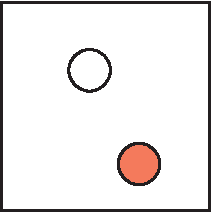
\includegraphics[width=1.5in]{figs/sample}
 \caption{Figure illustrating some proposed desgins.}
 \label{fig:sample}
\end{figure}

\subsection{Data}
\label{sec:data}

Describe the data and your access to it here.

\subsection{Evaluation}
\label{sec:eval}

Describe your plan for evaluating your work, even if it does not fit in the
timeframe of this project. Without time constraints, what would you? Do you
have the resources (people, time, equipment, data, money) to implement this
plan in the future?

\subsection{Timeline}
\label{sec:timeline}

Set up milestones for your project and  summarize in Table~\ref{tab:milestones}.

\begin{table}[h]
%% Table captions on top in journal version
 \caption{Project Milestones}\vspace{1ex} % the \vspace adds some space after the top caption
 \label{tab:milestones}
 \scriptsize
 \centering % avoid the use of \begin{center}...\end{center} and use \centering instead (more compact)
   \begin{tabular}{r|r}
     Date & Milestone (\%)\\
   \hline
     Sep 30 & Interviews conducted, initial task abstractions\\
     Oct  2 & Five datasets uploaded \\
     Oct  7 & Initial design sketches\\
     Oct 14 & Paper prototypes of 3 initial designs\\
     Oct 21 & Wireframe of central design \\
     Nov 7 & Initial prototype of design 
   \end{tabular}
\end{table}



\section{Impacts}
\label{sec:impact}

Although this is not a pioneering work, we think it does add to an academic advisor's arsenal for it considers grades more significantly than state-of-the-art.

We believe our main contribution is that this tool not only gives clustering of courses, but tells why two courses are clustered together in the parallel coordinates diagram. Existing course recommender system based on decision tree or neural network may not persuade users in a straight forward way how the conclusion is made. We use a simple yet convincing heurisitic.

We use parallel coordinates to show the trend in students' grades to indicate coursework content. This may inspire other researchers to study item similarity with this diagram.


%\bibliographystyle{abbrv}
\bibliographystyle{abbrv-doi-hyperref}
%%use following if all content of bibtex file should be shown
%\nocite{*}
\bibliography{proposal}
\end{document}

